\section{Error}

\subsection{Overview on error}
We can broadly classify the two key sources of error in CFD as follows:

\begin{itemize}
\item Numerical error:
	\begin{itemize}
	\item Solution error:
	This is evaluated at the when comparing the CFD simulation prediction value to those of the exact known solution value
	\item Truncation error:
	Formed when the actual governing equations (PDEs) are discretized into an approximate form for the numerical scheme
	\item Convergence error:
	They arise due to nature of the iterative technique used. Whether the residuals actually asymptote to machine-zero levels.
	\end{itemize}
\item Modeling error:
\begin{itemize}
	\item Sub-filter scale (SFS) turbulence model: 
		Since LES relies on modelling of the scales smaller than the filter size, then any inappropriate model selected would lead to over-/underprediction of the solution values
	\item Combustion and chemistry model:
		In LES we use the PCM-FPI to model to predict chemical reaction rates. If the model has an error, then this will reflect on the chemical kinetics.
    \item Aliasing errors occur when decomposed nonlinear terms in the FANS generate feedback of frequencies which are beyond the filter bandwidth, and eventually resolve as fictitious stresses
     \item Commutation errors exist between filtering and differential operations.
\end{itemize}
\end{itemize}
	
	
\subsection{Error estimation}
The basis for selective mesh refinement is the need to refine the mesh where the cells have a very critical effect on the solution, while coarsening the less critical areas to save on computational costs. There are two types of error estimation procedures available:
\begin{itemize}
\item a priori error estimators: these predict the long-term behavior of the errors in the discretization. They are not actually designed to approximate the error estimate for a given mesh. 
\item a posteriori error estimators: these use the simulation results to derive estimates of solution errors. Furthermore, these results are used to guide adaptive schemes:
\begin{itemize}
\item The mesh is locally refined ($h$-refinement) 
\item The degree of polynomial solution representation is raised ($p$-increment)
\end{itemize}
\end{itemize}
Two main a posteriori approaches are the:
\begin{itemize}
\item gradient-based: this is the more commonplace, and some useful discussions have been done by Giles and Pierce ~\cite{Giles:2000}
\item adjoint-based: this will be described in more detail in Section ~\ref{section:Adjoint}. Extensive work has been done by Giles and Pierce, ~\cite{Giles:2000}, Venditti and Darmofal ~\cite{Venditti:2000, Venditti:2002, Venditti:2003} Fidkowski and Darmofal: ~\cite{Fidkowski:2011} 
\end{itemize}


\subsection{Gradient-based refinement}

In these simulations, the mesh or discretization order is changed based on the rates of change of (physical) solution variables. The locations having the sharpest changes in solution quantities over a few mesh cells is flagged, and here the mesh resolution can be increased (higher mesh refinement), or the scheme order can be increased, effectively using a higher order discretization over these cells.

\begin{itemize}
\item The reasoning behind this is to have enough cells to capture the solution state changes so to represent them as \textit{smoothly} as possible.
\item Once refinement is completed, the solution is re-run and the gradients re-evaluated. Changes made as necessary. Error can be compared to a higher discretization ($h$ or $p$) solution.
\item This is the present utility in the anisotropic and isotropic AMR functionality of the CFFC code used by the CFD and Propulsion group.
\item As has been indicated in figure~\ref{fig:rhoError} the gradient-based approach does not guarantee error reduction for higher levels of $h$ refinement.
\end{itemize}


\begin{figure}[t!]
  \centering
   \subfigure[With isotropic AMR]{\label{fig:sphereIso}	   
   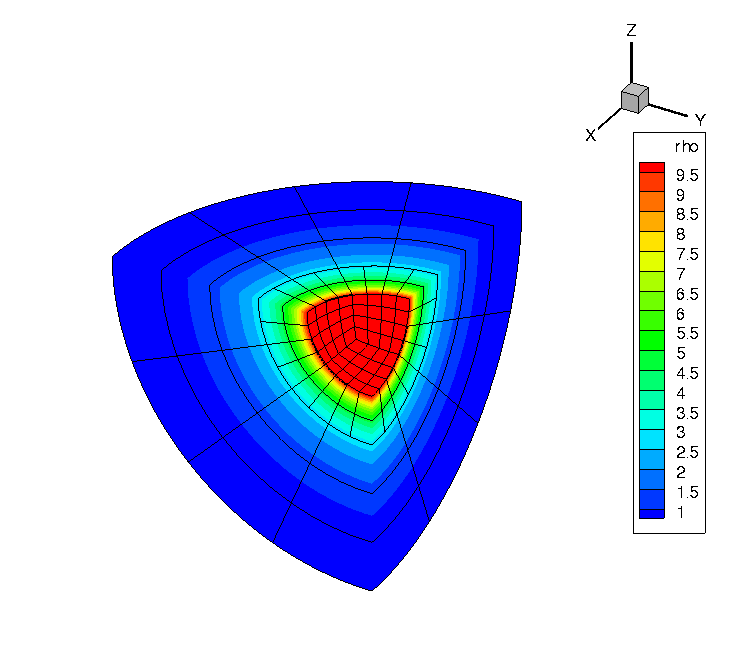
\includegraphics[width=0.2\textheight, trim=0cm 0cm 0cm 0cm,clip=true]{./figs/outflowIso.png}}%
   \:
   \subfigure[With anisotropic AMR]{\label{fig:sphereAniso}	   
   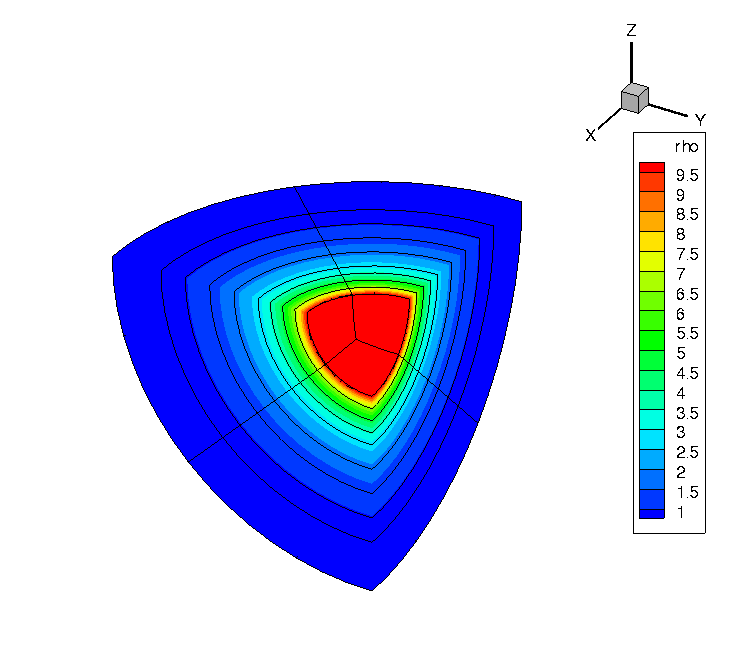
\includegraphics[width=0.2\textheight, trim=0cm 0cm 0 0cm,clip=true]{./figs/outflowAniso.png}}%
   \:
   \subfigure[Error in the density norm]{\label{fig:rhoError}	   
   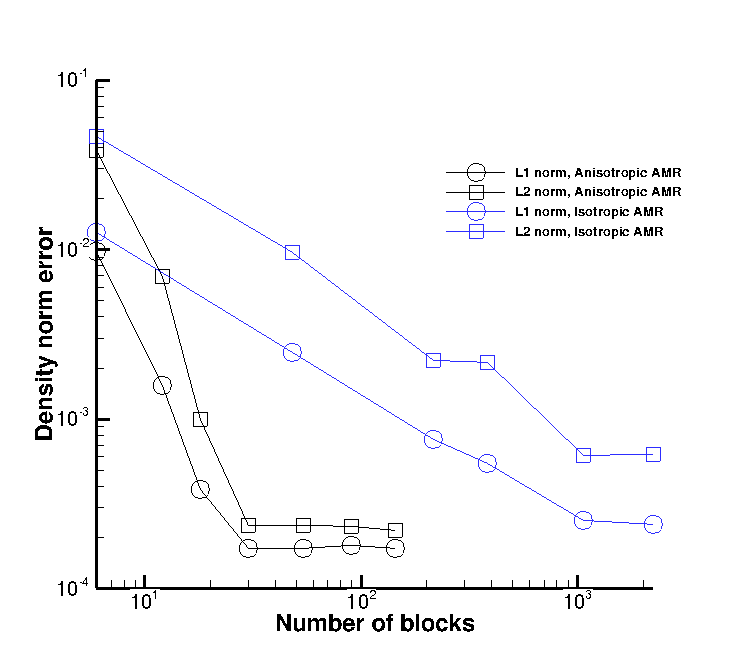
\includegraphics[width=0.2\textheight, trim=0cm 0cm 0 0cm,clip=true]{./figs/outflowError.png}}%
   \caption{Comparison of anisotropic and isotropic AMR and output error norms}  
   \label{fig:Gradientbased}
\end{figure}  


The number of cells to reach a convergence criteria is reduced in the case of figure \ref{fig:rhoError} by a factor of approximately $50$. Freret and Groth,~\cite{Freret:2015} and Williamschen and Groth~\cite{Williamschen:2013}.
A clear disadvantage is that for the gradient based approach, in spite of more mesh refinement, the error norm does not reduce. The graph reveals this asymptotic behavior of the convergence, yet for increased number of cells, there should be continual reduction in the density error norm.
